%% LaTeX Beamer presentation template (requires beamer package)
%% see http://bitbucket.org/rivanvx/beamer/wiki/Home
%% idea contributed by H. Turgut Uyar
%% template based on a template by Till Tantau
%% this template is still evolving - it might differ in future releases!

\documentclass[10pt]{beamer}


\usetheme{Malmoe}

\setbeamercovered{transparent}


\addtobeamertemplate{navigation symbols}{}{%
\usebeamerfont{footline}%
\usebeamercolor[fg]{footline}%
\hspace{1em}%
\insertframenumber/\inserttotalframenumber
}

\useoutertheme{infolines}
\setbeamertemplate{footline}{} 

\usepackage[brazil]{babel}
\usepackage[utf8]{inputenc}
\usepackage{listings}
\usepackage{mathptmx}
\usepackage[scaled=.90]{helvet}
\usepackage{courier}
\usepackage{url}
\usepackage{algorithm}
\usepackage{algpseudocode}


\usepackage[T1]{fontenc}

\title{Simulação de \textit{tracking} da dinâmica dos elétrons em um acelerador
síncrotron}

%\subtitle{}

% - Use the \inst{?} command only if the authors have different
%   affiliation.
%\author{F.~Author\inst{1} \and S.~Another\inst{2}}
\author{Gustavo Ciotto Pinton - RA 117136}

% - Use the \inst command only if there are several affiliations.
% - Keep it simple, no one is interested in your street address.
\institute
{

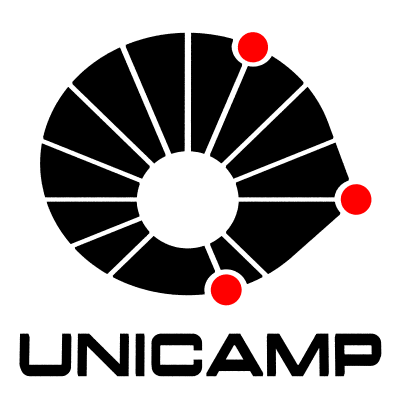
\includegraphics[scale=0.12]{logo} \\
\vspace{16pt}
Universidade Estadual de Campinas - UNICAMP\\
MO644 - Introdução à Computação Paralela}

\date{\today}


% If you wish to uncover everything in a step-wise fashion, uncomment
% the following command:

%\beamerdefaultoverlayspecification{<+->}

\begin{document}

%1
\begin{frame}
\titlepage
\end{frame}

\section{Introdução}
\begin{frame}
\frametitle{Introdução}

\begin{columns} %
\begin{column}{0.5\textwidth} %
	\begin{itemize}
	  \item Conjunto de vetores \(X^{i,j}_0\) representando estados de elétrons.
	  \vspace{12pt}
	  \item Elétrons submetidos a \(M\) atuadores em \(N\) voltas.
	  \vspace{12pt}
	  \item Simular quais vetores \(X^{i,j}_0\) atenderão a determinadas condições
	  ao fim de \(N * M\) iterações.
	\end{itemize}
\end{column} %
\begin{column}{0.5\textwidth}
     \begin{figure}
  \centering
  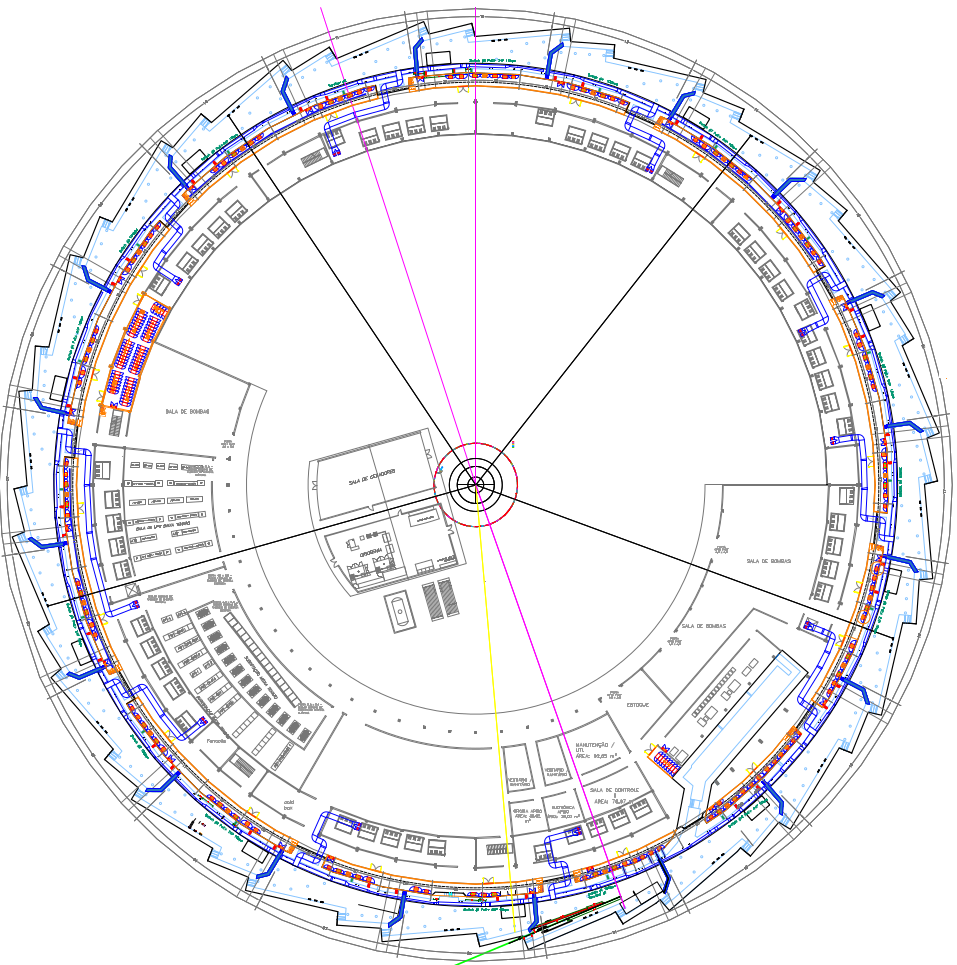
\includegraphics[width=\linewidth]{img/sirius}
  \caption{Acelerador \textit{Sirius}}
  \label{fig:speedup}
\end{figure}  
      
\end{column}
\end{columns}

\end{frame}

%2
\section{Análise do programa sequencial}
\begin{frame}
\frametitle{Programa sequencial}
\framesubtitle{\textit{Profiling}}

\begin{itemize}
  \item Utilização do \textbf{gprof}.
  \item Análise \textit{flat profile}: quanto tempo o programa gastou em cada
  função e quantas vezes tal função foi chamada.
  \item  97.43\% de todo o tempo gasto pelo programa está concentrado em apenas
  6 funções, todas chamadas dentro de \texttt{dynamical\_aperture\_search()}.
\end{itemize}

\vspace{-12pt}

\begin{table}[h]
    \centering
    \footnotesize
	\caption{\label{tab:flat} Análise \textit{flat profile} da execução sequencial.}
	\begin{tabular}{| c | c | c | c | c | }
		\hline
		\textbf{\% time} & \textbf{cum. sec.} & \textbf{self sec.} &
		\textbf{calls} & \textbf{name} \\ \hline 
		28.87 & 2.27 & 2.27  & 100000  & DynamicSearch::\textbf{performOneTurn(double
		(\&))} \\\hline 15.77 & 3.51 & 1.24  & 1200000020 & std::vector\(<\)RingElement\(>\)::\textbf{size()} const \\\hline 
		15.58 & 4.74 & 1.23  & 400000000  & Drift::\textbf{pass(double (\&))} \\\hline
		14.12 & 5.85 & 1.11  & 400000000  & Quadrupole::\textbf{pass(double (\&)} \\\hline
		11.64 & 6.77 & 0.92  & 200000000  & Sextupole::\textbf{pass(double (\&)} \\\hline
		11.45 & 7.67 & 0.90  & 100000000  & std::vector::\textbf{operator[]}(unsigned
		long) \\\hline \ldots & & & & \\\hline
	\end{tabular}
\end{table}

\end{frame}

%3
\begin{frame}
\frametitle{Programa sequencial}
\framesubtitle{\textit{Doacross e Doall loops}}

\begin{itemize}
  \item Laços externos são \textit{doall}: uma condição inicial \(X_0^{m,n}\)
  não depende de outra \(X_0^{m,p}\).
  \item Laços internos são \textit{doacross}: 
  \begin {itemize}
    \item Volta de índice \(i\) necessita dos resultados que as voltas \(i
    - 1, i - 2, \ldots, 0\).
	\item Estado \(X_{m}^{i,j}\) após atuador \(M_i\) necessita dos
	estados  \(X_{m-1}^{i,j}, \ldots, X_{0}^{i,j} \) .
	\end{itemize} 
\end{itemize}

\vspace{-12pt}

\begin{algorithm}[H]
\caption{Pseudo-código do algoritmo sequencial} 
\begin{algorithmic}[1]
  \Function{default\_dynamicSearch}{}
 	\For{$(i, j)$ in ${\mathbb{I}_x \times \mathbb{I}_y}$}
	    \State ${X^{i,j}} \gets f(i,j) $ \Comment{Calcula condição inicial \(X^{i,j}\) em função de \(i\) e \(j\)}
	    \For{$n \gets 0$ to ${N}$} \Comment{Itera sobre o número de voltas (\textbf{performOneTurn()})}
	        \For{$m \gets 0$ to ${M}$} \Comment{Itera sobre o número de atuadores (\textbf{size()})} 
	        \State $X^{i,j} \gets g_{A[m]} (X^{i,j})$
	        \Comment{Altera \(X_i\) de acordo com atuador \(A[m]\) (\textbf{pass()})}
	    	\EndFor
	    \EndFor
	\EndFor
   \EndFunction
\end{algorithmic}
\end{algorithm}

\end{frame}

%4
\section{Paralelização}
\subsection{Implementação}

\begin{frame}
\frametitle{Paralelização}
\framesubtitle{Implementação}
\begin{itemize}
  \item Distribui-se a computação de cada condição inicial \(X_0^{m,n}\) em uma
  \textit{thread} distinta: paralelização dos \textit{doall loops}.
  \item Cada \textit{thread} executa os \textit{doacross loops}.
  \item  Blocos de dimensões \(32\times32\), visto que a quantidade máxima
  de \textit{threads} por bloco é 1024.
  \item Maximizar o uso de um SM: para a \textit{NVIDIA Tesla K40c}, de
  \textit{compute capability 3.5}, o número máximo de warps por SM é 64,
  totalizando 2048 threads.
  \item Dois blocos inteiros por \textit{SM}.
\end{itemize}

\end{frame}

%5
\begin{frame}
\frametitle{Paralelização}
\framesubtitle{Implementação}

\begin{algorithm}[H]
\caption{Pseudo-código do kernel que é executado pela GPU} 
\begin{algorithmic}[1]
  \Function{dynamicSearchKernel}{$A,M,N,R$}
  	\State ${i} \gets \text{blockDim.y} * \text{blockIdx.y} + \text{threadIdx.y} $ \Comment{Índice y da \textit{thread}} 
  	\State ${j} \gets \text{blockDim.x} * \text{blockIdx.x} + \text{threadIdx.x} $ \Comment{Índice x da \textit{thread}}  
    \State ${X_i} \gets f(i,j) $ \Comment{Calcula condição inicial \(X_i\) em função de \(i\) e \(j\)}
    \For{$n \gets 0$ to ${N}$} \Comment{Itera sobre o número de voltas}
        \For{$m \gets 0$ to ${M}$} \Comment{Itera sobre o número de atuadores}
        	\State $X_i \gets g_{A[m]} (X_i)$ \Comment{Altera \(X_i\) de acordo com atuador \(A[m]\)}
    	\EndFor
    \EndFor
    \State ${R[i,j]} \gets X_i $ \Comment{Armazena resultado calculado}
   \EndFunction
\end{algorithmic}
\end{algorithm}

\end{frame}

%6
\subsection{Resultados}

\begin{frame}
\frametitle{Paralelização}
\framesubtitle{Resultados}

\begin{itemize}
  \item Testes no \textit{parsusy}: \textit{Intel(R) Xeon(R) E5-2620 v4} e
  \textit{NVIDIA Tesla K40c}.
  \item \textit{Flags} \texttt{gcc}: \texttt{-O3}, \texttt{-Wall},
  \texttt{--std=c++11}, \texttt{-mfpmath=sse} e \texttt{-sse2}.
  \item Duas implementações paralelas realizadas: uma com suporte a instruções
  \textit{FMA} (um arredondamento) e a outra compatível com a aplicação
  sequencial (dois arredondamentos).
\end{itemize}

\begin{figure}
  \centering
  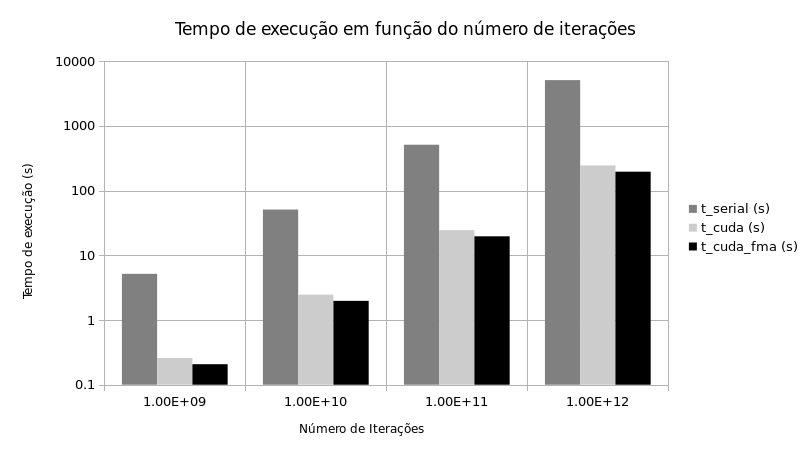
\includegraphics[width=0.55\linewidth]{img/time}
  \caption{Tempos de execução para diversos valores de \(N\)}
  \label{fig:time}
\end{figure}

\end{frame}

%7
\begin{frame}
\frametitle{Paralelização}
\framesubtitle{Resultados}


\begin{itemize}
  \item Em média, a solução que utiliza \textit{FMA} tem um
\textit{speedup} de \textbf{26.821}, enquanto que a tradicional,
\textbf{20.622}.
\end{itemize}

\begin{figure}
  \centering
  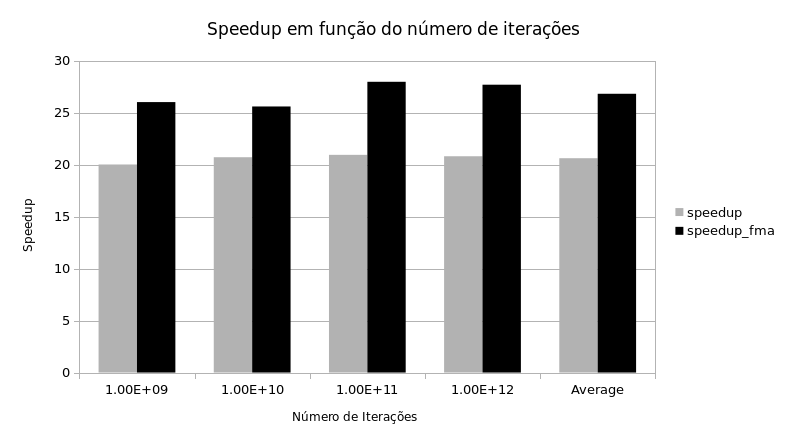
\includegraphics[width=0.70\linewidth]{img/speedup}
  \caption{\textit{Speedup} para diversos valores de \(N\)}
  \label{fig:speedup}
\end{figure}

\end{frame}

%8
\subsection{Dificuldades}
\begin{frame}
\frametitle{Paralelização}
\framesubtitle{Dificuldades}


\begin{itemize}
  \item \textit{It is not allowed to pass as an argument to a \path{__global__}
  function an object of a class derived from virtual base classes.} [NVIDIA.
  C/C++ language support]

  \item GPUs com \textit{compute capability} \(\ge2.0\): operação denominada
  \textit{fused-multiply-add} (\textit{FMA}) em pontos flutuantes de precisão
  simples e dupla.
  \item  Executar uma multiplicação e uma adição, isto é, computar \(X * Y +
  Z\), através de uma única instrução.
  \item Ganho em performance por executar duas operações de uma única vez.
  \item Realiza um arredondamento a menos que uma operação de multiplicação
  seguida por uma de adição.
  \item \(rn(X*Y+Z) \ne  rn(rn(X*Y) + Z)\). 
\end{itemize}

\end{frame}

\section{Referências}
\begin{frame}
\frametitle{Referências}

\begin{itemize}
\item Monniaux, D. (2008). The pitfalls of verifying floating-point computations. ACM Transactions on Programming Languages and Systems (TOPLAS).
\item NVIDIA. C/C++ language support. \url{http://docs.nvidia.com/cuda/cuda-c-programming-guide/index.html#virtual-functions}.
\item NVIDIA. Compute capabilities. \url{http://docs.nvidia.com/cuda/cuda-c-programming-guide/index.html#compute-capabilities}.
\item NVIDIA. Cuda C programming guide. \url{http://docs.nvidia.com/pdf/CUDA_C_Programming_Guide.pdf}.
\item Whitehead, N. and Fit-Florea, A. (2011). Precision performance: Floating point and IEEE 754 compliance for NVIDA GPUs. nVidia technical white paper.
\end{itemize}

\end{frame}
\end{document}